\documentclass[12pt,a4paper]{article}
\usepackage{amsmath}
\usepackage{amsfonts}
\usepackage{amssymb}
\usepackage[utf8]{inputenc}
\usepackage[T1, T2A]{fontenc}
\usepackage[english, russian]{babel}
\usepackage{graphicx}
\usepackage[left=2cm,right=2cm,top=2cm,bottom=2cm]{geometry}
\usepackage{calc}
\usepackage{wrapfig}
\usepackage{setspace}
\usepackage{indentfirst}
\usepackage{subfigure}
\usepackage{booktabs}
\usepackage[table,xcdraw]{xcolor}

\usepackage{fancybox}
\usepackage{fancyhdr}
\usepackage{ifthen}
\usepackage{pdfpages}
\usepackage[strict]{changepage}

\hyphenpenalty = 100000
\tolerance = 10000

%\setlength{\parindent}{0pt}

% for lab number change in all doc
\newcommand{\labnum}{
    2.3.1
}

% page style setup (for running titles)
\fancypagestyle{plain}{ %
    \fancyhf{} % remove everything
    
     % lines parameters
    \renewcommand{\headrulewidth}{0pt}
    \renewcommand{\footrulewidth}{0pt}
    
    % running titles contents
    \fancyfoot[L]{\ifthenelse{\isodd{\thepage}}{Работа \labnum}{\thepage}}
    \fancyfoot[R]{\ifthenelse{\isodd{\thepage}}{\thepage}{Работа \labnum}}
}

% choosing page style with our running titles
\pagestyle{plain}

\newcommand{\tablIns}{$ \texttt{\textbf{p, торр}}\cdot 10^{-4} $}

\title{
Отчет о выполнении лабораторной работы \labnum \\
Получение и измерение вакуума
}

\author{Матренин Василий, Б01-006}

\begin{document}
\maketitle

\paragraph{Цель работы:} 1) измерение объемов форвакуумной и высоковакуумной частей установки; 2) определение скорости откачки системы в стационарном режиме, а также по ухудшению и улучшению вакуума.
\paragraph{В работе используются:} вакуумная установка с манометрами: масляным, термопарным и ионизационным.

\section{Теоретическая часть}
\subsection*{Экспериментальная установка}
В данной работе используются традиционные методы откачки механическим форвакуумным насосом до давления $10^{-2}$ торр и диффузионным масляным насосом до давления $10^{-4}$ торр.

Установка изготовлена из стекла,
и состоит из форвакуумного баллона (ФБ), высоковакуумного диффузионного насоса (ВН), высоковакуумного баллона (ВБ), масляного (М) и ионизационного (И) манометров, термопарных манометров ($\text{М}_1$ и $\text{М}_2$), форвакуумного насоса (ФН) и соединительных кранов ($K_1, K_2,..., K_6$) (рис. 1). Кроме того, в состав установки входят: вариатор
(автотрансформатор с регулируемым выходным напряжением), или
реостат и амперметр для регулирования тока нагревателя диффузионного насоса. \\
\begin{figure}[!h]
    \centering
    \includegraphics[width=0.4\linewidth]{"picks/Схема установки"}
    \caption[]{Схема установки}
    \label{fig:Схема установки}
\end{figure}

Все краны вакуумной установки стеклянные. Стенки кранов тонкие, пробки кранов \mbox{полые} и составляют одно целое с рукоятками. Пробки кранов притерты к корпусам. Для герметизации используется вакуумная смазка.

\newpage

Устройство и принцип действия \textit{форвакуумного насоса} схематически, но довольно ясно изображены на рис 2. В положениях <<а>> и <<б>> пластина <<А>> засасывает разреженный воздух из откачиваемого объёма, а пластина <<Б>> вытесняет ранее захваченный воздух в атмосферу. В положениях <<в>> и <<г>> пластины поменялись ролями.
\begin{figure}[!h]
    \centering
    \includegraphics[width=0.85\linewidth]{"picks/устройство фв насоса"}
    \caption[]{Схема действия ротационного двухпластинчатого форвакуумного насоса}
    \label{fig:Схема ФВ насоса}
\end{figure}

Устройство и принцип действия \textit{диффузионного насоса} схематически изображены на рис 3. Такой насос работает в тысячи раз быстрее форвакуумного. Его действие основано на диффузии. Масло, налитое в сосуд А, подогревается электрической печкой. Пары масла поднимаются по трубке Б и вырываются из сопла В. Струя паров увлекает молекулы газа, которые поступают из откачиваемого сосуда через трубку ВВ. В трубке Г мало осаждается и стекает вниз. Оставшийся газ, выходя в трубку ФВ, откачивается форвакуумным насосом. \\
\begin{figure}[!h]
    \centering
    \includegraphics[width=0.4\linewidth]{"picks/устройство вв насоса"}
    \caption[]{Схема работы диффузионного насоса}
    \label{fig:Схема ВВ насоса}
\end{figure}

Диффузионный насос работает наиболее эффективно, когда длина свободного пробега молекул примерно равна ширине кольцевого зазора между соплом В и стенками трубки ВВ. Давление насыщенных паров масла при рабочей температуре, создаваемой обогревателем сосуда А, много больше $5\cdot 10^{-2}$ торр, поэтому пары масла создают плотную струю, увлекающую с собой молекулы газа.

Диффузионный насос, используемый в нашей установке (см. рис 1) имеет две ступени и соответственно два сопла. Одно сопло вертикальное (первая ступень), второе горизонтальное (вторая ступень). За второй ступенью имеется ещё одна печь, но пар из этой печи поступает не в сопло, а по тонкой трубке подводится ближе к печке первой ступени. Эта печь осуществляет фракционирование масла. Легколетучие фракции масла, испаряясь, поступают в первую ступень, обогащая её. По этой причине плотность струи первой ступени выше, и эта ступень начинает откачивать при более высоком давлении в форвакуумной части. Вторая ступень обогащается малолетучими фракциями масла. Плотность струи второй ступени меньше, но меньше и давление насыщенных паров. Соответственно, в откачиваемый объем поступает меньше паров масла, и его удаётся откачать до более высокого вакуума.  \\
\begin{wrapfigure}{r}{50mm}
    \begin{center}
    \includegraphics[width=0.9\linewidth]{"picks/термопара"}
        \caption{Схема термопарного манометра с лампой ЛТ-2}
        \label{fig:Схема термопары}
    \end{center}
\end{wrapfigure}

\textit{Термопарный манометр.} Чувствительным элементом манометра является платиново-родиевая термопара, спаянная с никелевой нитью накала и заключённая в стеклянный баллон. Устройство термопары пояснено на рис. 4. По нити накала НН пропускается ток постоянной величины. Для установки тока служит потенциометр R, расположенный на передней панели вакуумметра. Термопара ТТ присоединяется к милливольтметру, показания которого определяются \linebreak температурой нити накала и зависят от отдачи тепла в окружающее пространство. \\

Потери тепла определяются теплопроводностью нити и термопары, теплопроводностью газа, переносом тепла конвективными потоками газа внутри лампы, и \linebreak теплоизлучением нити (инфракрасное тепловое излучение). В обычном режиме лампы основную роль играет \linebreak теплопроводность газа. При давлениях, не меньших 1 торр, теплопроводность газа, а вместе с ней и ЭДС термопары практически не зависят от давления газа, и прибор не работает. \\

При улучшении вакуума средний свободный пробег молекул становится сравнимым с диаметром нити, \linebreak теплоотводность падает, и температура спая возрастает. При вакууме порядка $10^{-3}$ торр теплоотвод, осуществляемый газом, становится сравнимым с другими потерями тепла, и температура становится практически постоянной. Градуировочная кривая термопары приведена на рис. 5. \\
\begin{figure}[!h]
    \centering
    \includegraphics[width=0.3\linewidth]{"picks/градуировочная кривая"}
    \caption[]{Градуировочная кривая термопары ЛТ-2}
    \label{fig:Градуировочная кривая}
\end{figure}
\newpage
\begin{wrapfigure}{r}{60mm} %если не лезет, но с новой стр
    \begin{center}
        \includegraphics[width=60mm]{"picks/лампа"}
        \caption{Схема ионизационной лампы ЛТ-2}
        \label{fig:лампа}
    \end{center}
\end{wrapfigure}
\textit{Ионизационный манометр.} Схема ионизационного манометра изображения на рисунке 6. Он представляет собой трехэлектродную лампу. Электроны испускаются раскалённым катодом и увлекаются электрическим полем к аноду, имеющему вид редкой спирали. Проскакивая за её витки, электроны замедляются полем коллектора и возвращаются к аноду. Прежде чем осесть на аноде, они успевают много раз пересечь пространство между катодом и коллектором. На своём пути электроны ионизуют молекулы газа. Ионы, образовавшиеся между анодом и коллектором, притягиваются полем коллектора и определяют его ток. \\

Накалённый катод ионизационного манометра \linebreak перегорает, если давление в системе превышает $10^{-3}$ торр, поэтому перед его включением необходимо проверить давление термопарным манометром. \\
\subsection*{Процесс откачки}
\noindentОпишем процесс откачки математически: \\

Пусть W --- объем газа, удаляемого из сосуда при данном давлении за единицу времени, $Q_i$ для различных значений i обозначим различные притоки газа в сосуд (в единицах PV), такие как течи извне $Q_\text{и}$, десорбция с поверхностей внутри сосуда $Q_\text{д}$, обратный ток через насос $Q_\text{н}$. Тогда, приравнивая убыль газа из сосуда (с точностью до $RT/\mu$) в единицу времени $-VdP$ и сумму перечисленных токов имеем:
\begin{equation}
    -VdP = (PW - \sum_i Q_i)dt
\end{equation}
При достижении предельного вакуума устанавливается давление $P_{\text{пр}}$, и $dP = 0$. Тогда
\begin{equation}
W = ( \sum_i Q_i )/P_{\text{пр}}
\end{equation}
Поскольку обычно $Q_\text{и}$ постоянно, а $Q_\text{н}$ и $Q_\text{д}$ слабо зависят от времени, также считая постоянной W, можем проинтегрировать (1) и получить:
\begin{equation}
    P - P_{\text{пр}} = (P_0 - P_{\text{пр}})\exp(-\frac{W}{V}t)
\end{equation}
Полная скорость откачки $W$, собственная скорость откачки насоса $W_{\text{н}}$ и проводимости элементов системы $C_1, C_2,...$ соотносятся согласно формуле (4), и это учтено в конструкции установки.
\begin{equation}
\frac{1}{W} = \frac{1}{W} + \frac{1}{C_1} + \frac{1}{C_2} + ...
\end{equation}

\newpage

\subsection*{Течение газа через трубу}
Характер течения газа существенно зависит от соотношения между размерами системы и длиной свободного пробега молекул. При атмосферном и форвакуумном давлениях  длина свободного пробега меньше диаметра трубок, и течение газа определяется его вязкостью, т.е. взаимодействием молекул. При высоком вакууме течение существеннее определяется взаимодействием со стенками \\
Для количества газа, протекающего через трубу длины $l$ и радиуса $r$ в условиях высокого вакуума, справедлива формула:
\begin{equation}
    \frac{d(PV)}{dt} = \frac{4}{3}r^3\sqrt{\frac{2\pi RT}{\mu}}\frac{P_2 - P_1}{l}
\end{equation}
Если труба соединяет насос установку, то давлением $P_1$ у насоса можно пренебречь. Давление в сосуде $P = P_2$. Тогда имеем:
\begin{equation}
C_\text{тр} = \left(\frac{dV}{dt}\right)_\text{тр} = \frac{4r^3}{3l}\sqrt{\frac{2\pi RT}{\mu}}
\end{equation}
Для пропускной способности отверстий имеется формула
\begin{equation}
C_\text{отв} = \left(\frac{dV}{dt}\right)_\text{отв} = S\frac{\bar{\upsilon}}{4}
\end{equation}
Для воздуха при комнатной температуре $\bar{\upsilon}/4 = 110~\text{м/с} = 11~\text{л/c}\cdot\text{см}^2$.

\newpage

\section{Ход работы}

\subsection*{Измерение объёмов форвакуумной и высоковакуумной частей установки}
    \begin{enumerate}
        \item Проверил, что $K_4$ открыт, впустил в установку атмосферный воздух через краны $K_1$ и $K_2$. <<Запер>> в капилляре атмосферный воздух кранами $K_5$ и $K_6$. Объем капилляра в используемой установке - $V_\text{к} = 50~ \text{см}^3.$
        \item Закрыл $K_1$ и $K_2$, включил форвакуумный насос и дал ему откачать себя. Подключил установку к насосу краном $K_2$. Откачал установку до $10^{-2}$ торр. Отсоединил установку краном $K_2$, и оставил насос работать <<на себя>>. Перекрыл  $K_3$, отделяя высоковакуумною часть установки. Закрыл $K_4$, чтобы привести в готовность масляный манометр.
        \item Открыл  $K_5$, чтобы <<запертый>> ранее воздух заполнил форвакуумную часть установки, снял давление с помощью вакуумного манометра, измерив разность высот столбиков масла:
        $$
        \Delta h = (29.0\pm0.1) ~\text{см}
        $$
        \item Из того, что плотномть плотность масла в манометре равна 885 г/л, и считая, что установившееся давление много больше форвакуумного, получил:
        $$
        P = (2518\pm18)~\text{Па}
        $$
        Из уравнения состояния (изотерма) :
        $$
        V_\text{ФВ} = (1950\pm15)~\text{см}^3
        $$
        \item Открыв кран $K_3$, получил значение разности высот на манометре (аналогично) :
        $$
        \Delta h = (18.7\pm0.1) \text{см}
        $$
        Получил объем высоковакуумной части установки (погрешности сложились):
        $$
        V_\text{ВВ} = (1100\pm30)~\text{см}^3
        $$
        \item Открыл кран $K_4$.
    \end{enumerate}

\newpage

\subsection*{Получение высокого вакуума}
    \begin{enumerate}
    \item Откачал установку ФВ насосом.
    \item Включил термопарные манометры, устанавил их токи согласно паспортам. Переключил прибор в режим измерения ЭДС и определил давление в установке по градуировочной кривой (рис. 5)
    \item По достижении форвакуума закрываем $K_6$ и начинаем откачку высоковакуумного баллона с помощью диффузионного насоса
    \item Включив ионизационную лампу, производим обезгаживание и записываем минимальное установившееся давление:
    $$P_{\text{пр}} = 6,0\cdot10^{-5} ~\text{торр}$$    
\end{enumerate}

\newpage

\subsection*{Измерение скорости по ухудшению и улучшению вакуума}
\begin{enumerate}
    \item Закрываем кран $K_3$, отключая тем самым откачку вакуума и записываем на видео изменения показаний микроамперметра, пока вакуум не ухудшится до $7,6\cdot10^{-4}$ торр. Затем открываем $K_3$ и так же записываем улучшение вакуума. Приводим результаты повторных измерений в таблице 1 и на графиках (рис. 7 и 8).
    \begin{table}[!h]
        \centering
        \resizebox{0.9\textwidth}{!}{%
            \begin{tabular}{|c|c|c|c|c|c|c|c|c|c|}
                \hline
                \multicolumn{2}{|c|}{{ \textbf{Улучшение,   1}}} & \multicolumn{2}{c|}{{ \textbf{Улучшение, 2}}} & \multicolumn{2}{c|}{{ \textbf{Ухудшение, 1}}} & \multicolumn{2}{c|}{{ \textbf{Ухудшение, 2}}} & \multicolumn{2}{c|}{{ \textbf{Ухудшение, 3}}} \\ \hline
                t, с  & \tablIns  & t, с & \tablIns  & t, с & \tablIns  & t, с & \tablIns  & t, с & \tablIns  \\ \hline
                0     &    7.60   &  0   &   7.60    &  0   &    0.65   &  0   &    0.71   &  0   &    0.76   \\ \hline
                1     &    6.50   &  1   &   7.00    &  5   &    0.76   &  5   &    0.72   &  5   &    1.20   \\ \hline
                2     &    5.50   &  2   &   5.50    &  10  &    1.20   &  10  &    1.10   &  10  &    1.70   \\ \hline
                3     &    4.60   &  3   &   4.30    &  16  &    1.70   &  15  &    1.60   &  15  &    2.20   \\ \hline
                5     &    3.10   &  4   &   3.60    &  25  &    2.50   &  21  &    2.20   &  20  &    2.70   \\ \hline
                8     &    1.90   &  5   &   2.90    &  35  &    3.30   &  31  &    3.10   &  29  &    3.60   \\ \hline
                13    &    1.10   &  10  &   1.40    &  45  &    4.10   &  41  &    4.00   &  39  &    4.50   \\ \hline
                18    &    0.83   &  15  &   0.94    &  55  &    5.00   &  51  &    4.90   &  49  &    5.50   \\ \hline
                23    &    0.74   &  18  &   0.85    &  75  &    6.70   &  66  &    6.30   &  59  &    6.40   \\ \hline
                37    &    0.70   &  26  &   0.76    &  84  &    7.50   &  79  &    7.50   &  71  &    7.50   \\ \hline
            \end{tabular}
        }
    \caption{Зависимости давления от времени}    
    \end{table}

    \begin{figure}[!h]
        \begin{center}
            \subfigure[Измерение 1]{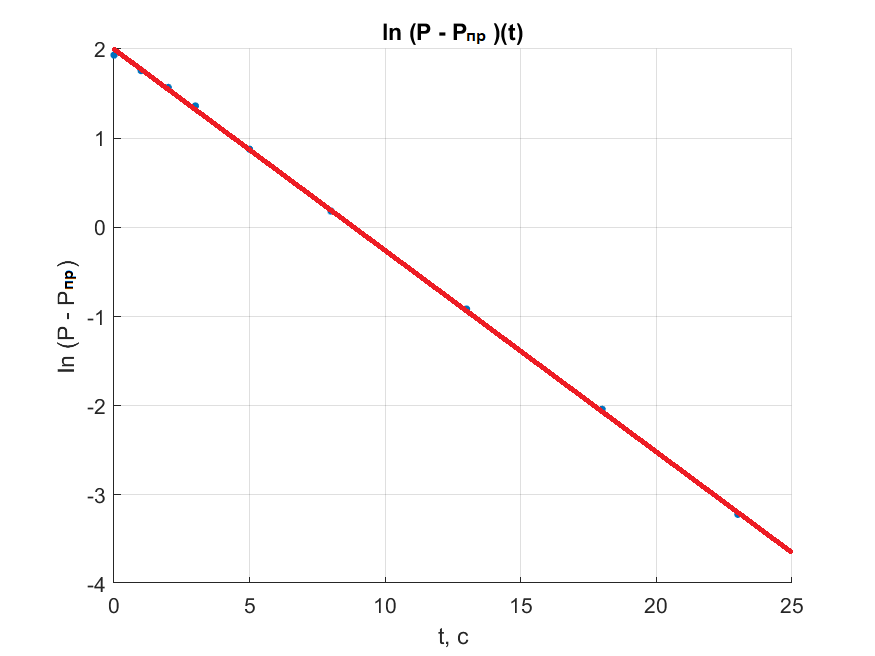
\includegraphics[width=0.45\textwidth]{"matlab/231_PH1.png"}}
            \subfigure[Измерение 2]{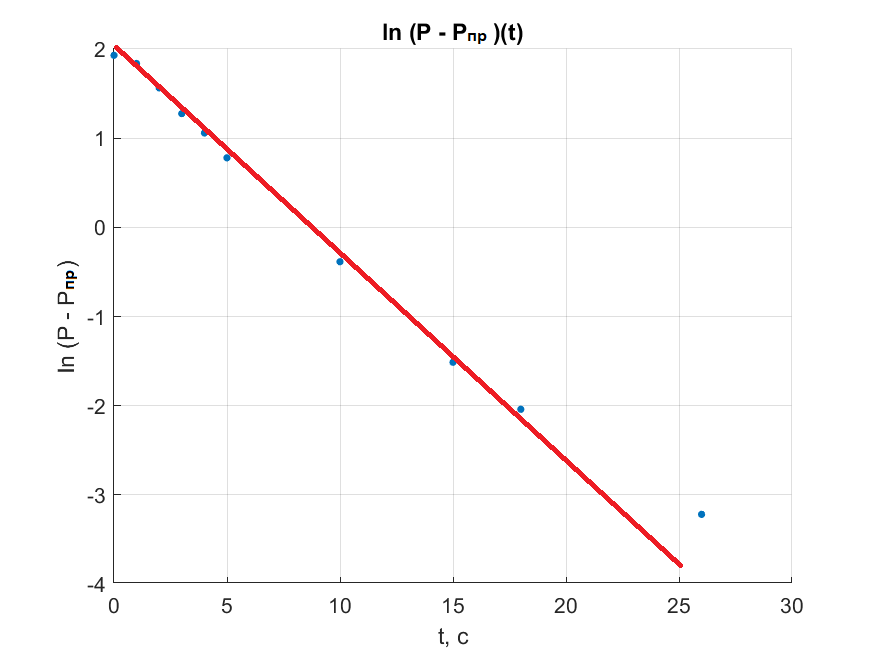
\includegraphics[width=0.45\textwidth]{"matlab/231_PH2.png"}}
        \end{center}
        \caption{Зависимость давления от времени по улучшении вакуума}
    \end{figure}

    \begin{figure}[!h]
        \begin{center}
            \subfigure[Измерение 1]{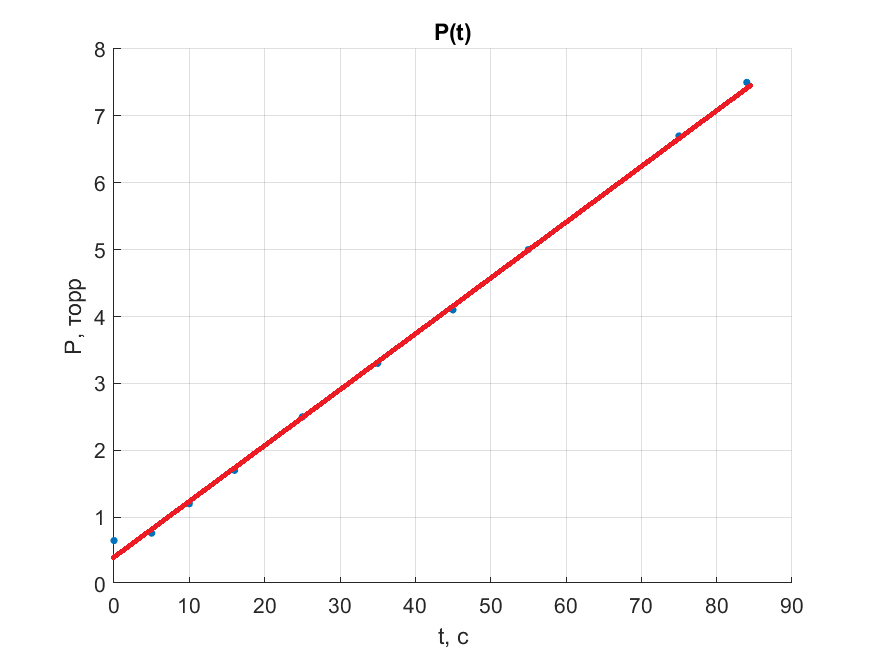
\includegraphics[width=0.3\textwidth]{"matlab/231_PL1.png"}}
            \subfigure[Измерение 2]{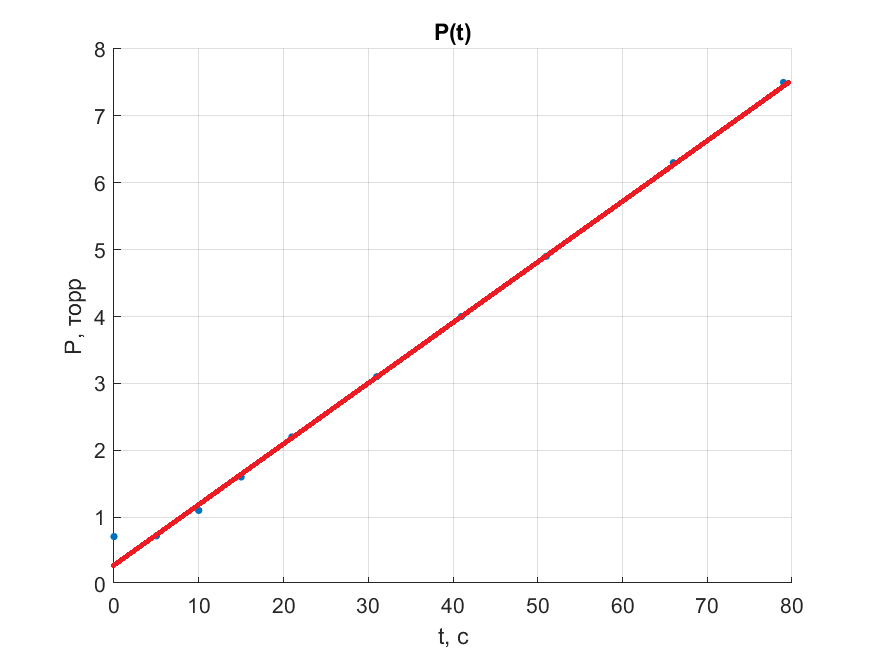
\includegraphics[width=0.3\textwidth]{"matlab/231_PL2.png"}}
            \subfigure[Измерение 3]{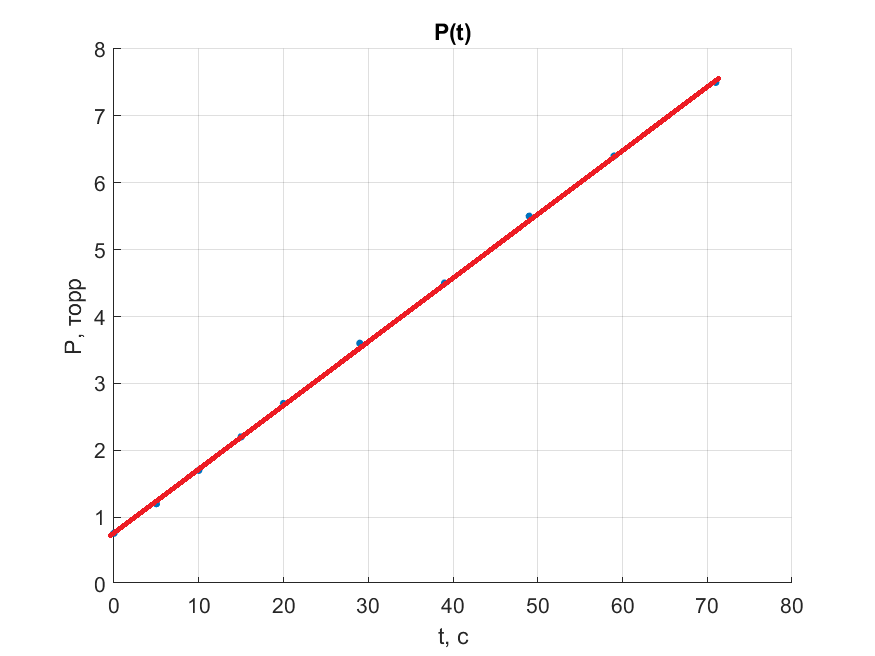
\includegraphics[width=0.3\textwidth]{"matlab/231_PL3.png"}}
        \end{center}
        \caption{Зависимость давления от времени по ухудшению вакуума}
    \end{figure}
    \item
    Рассчитав коэффициенты наклона графиков 7(а) и 7(б) и зная объем высоковакуумной части установки, получим скорость откачки W диффузионного насоса, сравнив графики с зависимостью (4). Считаем $$W = -\bar{a}\cdot V, \quad\varepsilon_W^2 = \varepsilon_{\bar{a}}^2 + \varepsilon_V^2, $$  где $\bar{a}$ --- среднее коэффициентов наклона из зависимостей 7(а) и 7(б). Имеем:
    $$W = (0,261\pm0,02) ~\text{л/с}$$
    \item
    Имея в виду соотношения (1) для случая ухудшения вакуума (без откачки), оценим $Q_\text{н}$ c помощью полученных зависимостей 8(а, б, в). Считаем $$\frac{dP}{dt} = \bar{a}$$ где $\bar{a}$ --- среднее коэффициентов наклона из зависимостей 8(а), 8(б), 8(в). Имеем:
    $$Q_\text{н} + Q_\text{д} = (1,21\pm0,05)\cdot 10^{-5} ~\text{торр}\cdot\text{л/c}$$
    $Q_\text{д}$ обычно порядка $10^{-8}$, поэтому можно считать $Q_\text{н} + Q_\text{д} \approx Q_\text{н}$. Таким образом,
    $$Q_\text{н} + Q_\text{д} \approx 1,26\cdot 10^{-5} ~\text{торр}\cdot\text{л/c}$$
    \item Оценим пропускную способность трубы от вакуумного баллона, имея в виду порядки её диаметра и длины и размерного множителя $$d \sim 10^{-2}~\text{м},\quad L \sim 1 ~\text{м},\quad \sqrt{\frac{RT}{\mu}} \sim 500 ~\text{м/с},$$ используя формулу (6) имеем:
    $$C_\text{тр} \sim 1 ~\text{л/с},$$
\end{enumerate}

\newpage


\section{Выводы}
\begin{enumerate}
    \item Проверены теоретические зависимости, связанные с течением газа (рис. 7 и 8)
    \item Измерено значение производительности насоса с точностью $\varepsilon = 8\%$
\end{enumerate}
\end{document}
